\chapter{Problems and Future Work}\label{prbftr}

In this chapter, some problems in the prediction results are presented in section \ref{prblms}, and the future directions are illustrated in section \ref{ftrwrk}.

\section{Problems}\label{prblms}

This section mainly shows the two existed problems in the prediction result, and proposes corresponding possible solutions. Subsection \ref{outres} shows the resolution problem causing the inaccurate prediction and subsection \ref{flsvtx} shows the false vertex problem.

\subsection{Output Resolution}\label{outres}
We know that the output grid for a single vertex has the resolution 28$\times$28. The input resolution of PolygonRNN is 224$\times$224. Thus, a single pixel in the output grid corresponds to an area of 8$\times$8 in the original image. This will result in inaccurate output vertices.

(Example)

The possible solution is to extract features from relatively shallow levels. However, these layers may not have much semantic information, which may further have negative effect on the prediction accuracy of RNN part. In addition, because of the presence of FC layer at the end of the output part of the RNN, the number of its weights would increase at the fourth power. For example, currently the FC layer has $(28\times28)^2$ weights, if we increase the resolution to 56$\times56$, the number of weights would be $(56\times56)^2$, 16 times the original. Therefore, the conclusion is that if the resolution is increased, then the network structure would certainly need to make a number of changes.

\subsection{False Vertex}\label{flsvtx}
Actually, after the introduction of beam search algorithm, the false vertex problem has been solved a lot and the prediction is greatly improved, but there are still some in the results.

(Example)

The possible solution comes from the point of view of geometry, penalizing the angle degree of the polygon. Figure \ref{fig:agldstb} shows the polygon interior angle degree distribution in the dataset of Zurich and Chicago.

\begin{figure}[!h]
	\centering
	\subbottom[angle distribution in Zurich\label{fig:agldstbzurich}]{
		\includegraphics[width=\figfig\textwidth]{5-02-0.pdf}
	}
	\subbottom[angle distribution in Chicago\label{fig:agldstbchicago}]{
		\includegraphics[width=\figfig\textwidth]{5-02-1.pdf}
	}
    \caption[Polygon interior angle distribution]{Polygon interior angle distribution.}
	\label{fig:agldstb}
\end{figure}

From figure \ref{fig:agldstbchicago} we can see that in Chicago, most angles are at $90^\circ$ or $270^\circ$, indicating that most of them are right angles. In Zurich's figure \ref{fig:agldstbzurich}, although most angles are around $90^\circ$ or $270^\circ$, they have certain deviations about $\pm20^\circ$. Also, there is a peak near $180^\circ$ in figure \ref{fig:agldstbzurich}, which means that there are many three-point collinearity in the dataset of Zurich.

When doing the probability computation of the next vertex, we can use the distribution of the angle as a priori to guide the prediction.

\section{Future Work}\label{ftrwrk}

In this section, several future directions are presented, such as possible direction of road segmentation, the improvement of the dataset, the methods that are helpful for training and the possible extensions of the model.

\paragraph{Road Segmentation}
At present, our project does not include road segmentation. This is because roads cannot usually be described in terms of polygons. We hope to add this in the future so that the geometrical segmentation in aerial images can become complete. The idea is to convert roads into centerlines and intersections. Actually, in Mask R-CNN, the part of human posture detection is doing this, where a person is structurized as several keypoints and edges that connect them. Figure \ref{fig:posdet} shows the human posture detection result of Mask R-CNN.
\begin{figure}[!h]
	\centering
	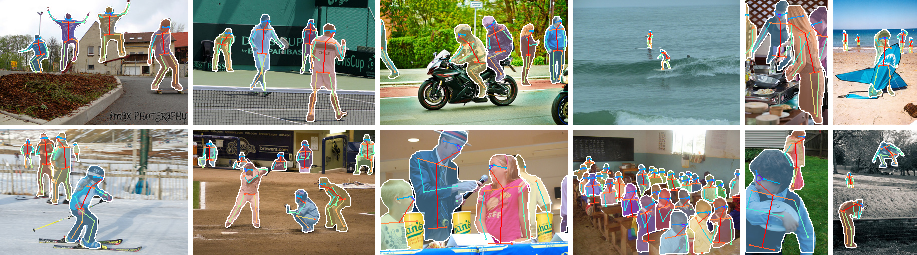
\includegraphics[width=\fig\textwidth]{5-03.pdf}
    \caption[Human posture detection in Mask R-CNN]{Human posture detection in Mask R-CNN. Image copyright owned by \cite{maskrcnn}.}
	\label{fig:posdet}
\end{figure}
However, it is difficult to apply this method to our project, because the road is different from the human body, the number of keypoints of roads in each image is not fixed. In addition, paper (XXX) uses incremental graph construction process, which may be possible to be used in our project.

\paragraph{Ground Truth Correction}
Subsection \ref{adjust} has already introduced a method to correct ground truth. However, there are still some image-polygon pairs inaccurate, especially for those adjacent buildings (see figure \ref{fig:egshi3}). We hope that dataset can be collected from single source, so that the polygons and the buildings are more likely to match each other. As for the adjacent buildings, it is difficult for us to merge their polygons into a single one. Thus, we hope polygons of buildings instead of houses can be provided.

\paragraph{RoIAlign Implementation}
Subsection \ref{algmod} has already introduced the hybrid version with RoIAlign of \modelnameshort. We hope that in the future this kind of version can be implemented.

\paragraph{Training Method}
Our model does not use pre-trained VGG-16 during training, neither as an initializer nor as fixed weights. As for training, in the future we hope the alternating training method can be introduced, just like what shows in the Fast R-CNN paper.

\paragraph{Model Generalization}
In fact, our model can be applied not only to the geometrical shape segmentation in the aerial images, but also to the general multi-object segmentation. We hope that our model \modelnameshort can be generalized to other fields and we can compare the performance under different dataset.

